\documentclass[11pt]{beamer}

%%%%%%%% tema e cor %%%%%%%%
\mode<presentation> {
\usetheme{Madrid}
\usecolortheme{rose}
}

\usepackage[english]{babel}
\usepackage[utf8]{inputenc}
\usepackage{graphicx} 
\usepackage{booktabs} 

%
%{
%================= logos no meio =====================
%\vspace*{-0.35cm}
%\includegraphics[width=1.8cm]{img/logo-uea.png}
%\hspace*{0.25cm}~%
%\includegraphics[width=1.8cm]{img/logo-neo.png}
%\vspace*{0.35cm}\\
%Núcleo de Engenharia e Otimização -- NEO \\
%Escola Superior de Tecnologia -- EST\\
%Universidade do Estado do Amazonas -- UEA\\
%%\medskip
%%\texttt{\{lods.eng,ronety\}@uea.edu.br} % emails
%}
\date{\today}

\AtBeginSection[]
{
\begin{frame}
\frametitle{Table of contents}
\tableofcontents[currentsection]
\end{frame}
}

%%%%%%%% Packages %%%%%%%%%
\usepackage{float}
\usepackage{subfig} %Subplots
\usepackage{graphicx}
\usepackage{hyperref}
\usepackage{enumerate}
\usepackage{amsmath}

%%%%%%%% title and subtitle %%%%%%%%
\title[ProbCons]{ProbCons: Probabilistic consistency-based multiple sequence alignment} 

%%%%%%%% name %%%%%%%%
\author[PCALG - Presentation]{Álvaro Huertas García \\ Diego Mañanes Cayero
                 \\ Alejandro Martín Muñoz \\ Sara Dorado Alfaro} 

\begin{document}

\frame{\titlepage}
\begin{frame}
    \frametitle{Table of contents}
    \tableofcontents
\end{frame}

%%%%%%%% slides %%%%%%%%

\section{Introduction} 
\begin{frame}{Introduction $\rightarrow$ 2 Frequency dependent fitness}

    \begin{itemize}    
        \item Game theory.
        \item $OncoSimulR$ model $\rightarrow$ the fitness of a subpopulation will depend on the relative abundance of the different subpopulations.
        \item The fitness of each subpopulation is defined as an arbitrary function of the genetic interactions between multiple genes.       
    \end{itemize}
    
\end{frame}

\begin{frame}{Introduction $\rightarrow$ Effects on fitness}

    \begin{itemize}
        \item $allFitnessEffects$ function:
        \begin{itemize}
            \item $genoFitness$ = dataframe
            \begin{itemize}
                \item First column: genotypes.
                \item Second column: expressions for the functions that relate fitness to frequencies of other genotypes.
            \end{itemize}
            \item $frequencyDependentFitness$ = TRUE
            \item $frequencyType$ = “rel” or $frequencyType$ = “abs”
            \item $spPopSizes$
        \end{itemize}        
    \end{itemize}

\end{frame}

\begin{frame}{Introduction $\rightarrow$ Assess fitness}

    \begin{itemize}
        \item $evalGenotype$ function:
        \begin{itemize}
            \item $fitnessEffects$ = $allFitnessEffects$ object
            \item $genotype$
        \end{itemize}
        \item $evalAllGenotypes$ function:
        \begin{itemize}
            \item $fitnessEffects$ = $allFitnessEffects$ object
        \end{itemize}
    \end{itemize}
    
\end{frame}

\begin{frame}{Introduction $\rightarrow$ Perform simulations}

    \begin{itemize}
        \item $oncoSimulIndiv$ and $oncoSimulPop$ functions.
    \end{itemize}
    \begin{columns}
        \begin{column}{0.5\textwidth}
            \begin{figure}[t]
                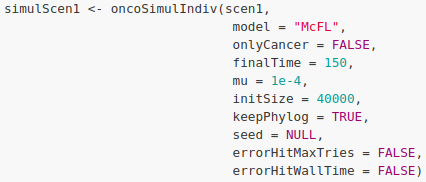
\includegraphics[width=0.9\linewidth]{img/oncoSimulIndiv.png}
            \end{figure}
        \end{column}
        \begin{column}{0.5\textwidth}
            \begin{figure}[t]
                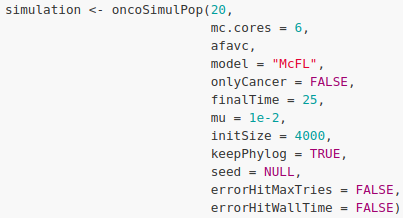
\includegraphics[width=0.9\linewidth]{img/oncoSimulPop.png}
            \end{figure}
        \end{column}
    \end{columns}
    
\end{frame}

\section{Consistency-based methods} 
\begin{frame}{Consistency-based methods}

    \begin{itemize}    
        \item Based on : “prevention is the best medicine”
        \item Combines iterative and progressive approaches with probabilistic models:
        \begin{enumerate}
        \renewcommand{\baselinestretch}{2}
        \item Uses \textbf{\underline{Hidden Markov Models}} to calculate matrices for matching residues in pairwise alignments. 
        \item Uses information about multiple sequence alignment as it is being generated to guide the pairwise alignments
        \item Multiple alignment via tree-based \textbf{\underline{progressive alignment}}
        \item Errors at early stages in the alignment are alleviated by \textbf{\underline{post-processing steps}} such as iterative refinement
        \end{enumerate}

    \end{itemize}
    
\end{frame}

\begin{frame}{Consistency-based methods}

    \begin{block}{Imaging this biological scenario}
    \centering
            \large Sequence x $\rightarrow$ $ x_{i}$ \\
            \large Sequence y $\rightarrow$ $ y_{i}$ \\
            \large Sequence z $\rightarrow$ $ z_{k}$ \\
    \end{block}
    \centering
    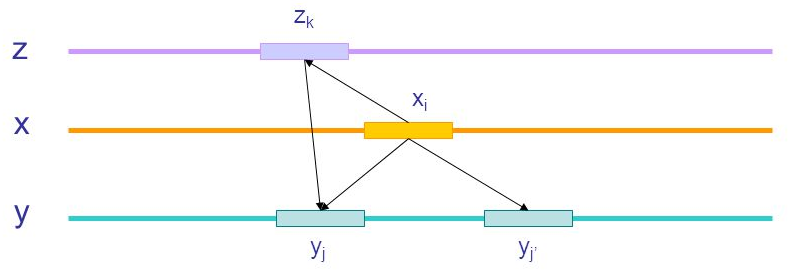
\includegraphics[width=0.65\linewidth]{img/xyz.PNG}
    \begin{itemize}
        \item If $ x_{i}$ aligns with $ z_{k}$ and $ z_{k}$ aligns with $ y_{i}$, then $x_{i}$ should align with $ y_{i}$
    \end{itemize}
    \begin{itemize}
            \item Consistency-based techniques \textbf{score pairwise alignments} in the context of \textbf{information about multiple sequences}
    \end{itemize}
\end{frame}

\section{ProbCons: The algorithm}
\begin{frame}{Algorithm overview}
    \begin{itemize}
        \item \textbf{ProbCons\cite{do2005probcons}} is a pair-hidden Markov model-based progressive alignment algorithm that differs from most typical approaches in its use of \textbf{maximum expected accuracy} rather than Viterbi alignment, and of the probabilistic consistency transformation to incorporate multiple sequence conservation information during pairwise alignment. 
        \item \textbf{Hidden Markov Models (HMMs)} in sequence analysis are based on a strong probabilistic model that \textbf{includes a representation of INDELs} (insertions and deletions, i.e. gaps). 
        \item The HMM describing families of related sequences are called \textbf{profile HMMs}
    \end{itemize}
\end{frame}

\begin{frame}{Algorithm overview}
    \begin{itemize}
        \item In profile HMMs the residues in each position of the alignment can be in one of three possible states:
        \begin{enumerate}
            \item \textbf{Match:} represent conserved position
            \item \textbf{Insert:} represent small stretches of nonspecific sequence
            \item \textbf{Delete:} correspond to gaps and represent the absence of a conserved residue
        \end{enumerate}
        \item Each state has associated:
        \begin{enumerate}
            \item \textbf{Emission probability:} correspond to the probability of observing each amino acid at that particular position of the alignment
            \item \textbf{Transition probability:} describes the frequency of observing a match, insertion or deletion in column i+1 given the state column i. 
        \end{enumerate}
    \end{itemize}
    
\end{frame}

\begin{frame}{Algorithm overview}
\centering
 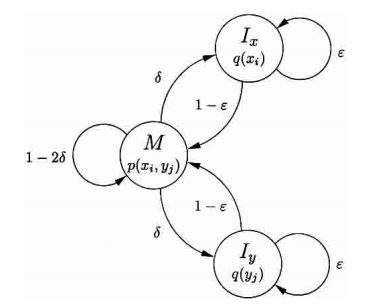
\includegraphics[width=0.35\linewidth]{img/hmm_states.PNG}
 \begin{itemize}
     \item Emission probabilities, which correspond to traditional substitution scores, are based on the BLOSUM62 matrix.
     \item Transition probabilities, which correspond to gap penalties, are trained with unsupervised Expectation-Maximization (EM)
     \begin{itemize}
         \item $\pi_{insert}$: initial insertion probability parameter
         \item $\delta$: insertion start probability parameter
         \item $\epsilon$: insertion extension probability parameter
     \end{itemize}
     \item The resulting parameters ($\delta$ = 0.019931, $\epsilon$ = 0.79433, $\pi_{insert}$= 0.19598) are used as the default for the program.

 \end{itemize}
    
\end{frame}

\begin{frame}
    \frametitle{Algorithm overview}

    \begin{block}{ProbCons \cite{do2005probcons}}
        \begin{itemize}
            \item Given $m$ sequences $\rightarrow$ $S = \{s^{(1)}, \ldots, s^{(m)} \}$.
            \item Maximum expected accuracy.
            \item Probabilistic consistency $\rightarrow$ MSA conservation information in the pairwise alignment.
        \end{itemize}
    \end{block}
    
    \begin{enumerate}
        \item Step 1: Computation of posterior probability matrices.
        \item Step 2: Computation of expected accuracies.
        \item Step 3: Probabilistic consistency transformation.
        \item Step 4: Computation of the guide tree.
        \item Step 5: Progressive alignment.
        \item Step 6: Iterative refinement (post-processing OPTIONAL step).
    \end{enumerate}
\end{frame}

\begin{frame}
    \frametitle{Step 1: Computation of posterior probability matrices}
    \begin{itemize}
        \item For $x, y \in S$, compute the matrix
        \begin{align*}
            P_{xy}(i,j) = \pmb{P}(x_i \sim y_j \in a^* | x, y) \;,
        \end{align*}
        where $1\leq i\leq|x|$ and $1\leq j\leq |y|$.
        \item Each position $P_{xy}(i,j)$ is the \textbf{posterior} probability that letters $x_i$ and $y_j$ are paired i an alignment $a^*$.
        \begin{itemize}
            \item Computing posterior probabilities in pair-HMMs \cite{durbin1998biological}.
        \end{itemize}
        \item Time complexity $O(m^2 L^2)$.
        \begin{itemize}
            \item $m$ is the number of sequences.
            \item $L$ is the length of each sequence.
        \end{itemize}
    \end{itemize}
\end{frame}

\begin{frame}
    \frametitle{Step 2: Computation of expected accuracies}
    \begin{itemize}
        \item The expected accuracy is defined as
        \begin{align*}
            \pmb{E}_{a^*} (acc(a,a^*)|x,y) = \frac{1}{\min{\{|x|,|y|\}}} \sum_{x_i\sim y_j \in a} P_{xy}(i,j) \;,
        \end{align*}
        where $a$ is the align*ment that maximizes the expected accuracy by dynamic programming.
        \item Set 
        \begin{align}\label{eq:score}
            E(x,y) = \pmb{E}_{a^*} (acc(a,a^*)|x,y) \;.
        \end{align}
    \end{itemize}
\end{frame}

\begin{frame}
    \frametitle{Step 3: Probabilistic consistency transformation}
    \begin{itemize}
        \item Reestimate quality scores $\pmb{P}_{xy}$ $\rightarrow$ probabilistic consistency transformation.
        \item Incorporate similarity of $x$ and $y$ to other sequences in $S$:
        \begin{align*}
            {\pmb{P}}'(x_i \sim y_j \in a^* | x, y) = \frac{1}{|S|} \sum_{z\in S} \sum_{z_k \in z} F(x_i, y_j, z_k) \;,
        \end{align*}
        where $F(x_i, y_j, z_k) =  {\pmb{P}}(x_i \sim z_k \in a^* | x, z) \times {\pmb{P}}(z_k \sim y_j \in a^* | z, y) $.
        \item In matrix form:
        \begin{align*}
            {P'}_{xy} = \frac{1}{|S|} \sum_{z\in S} P_{xz}P_{zy} \;.
        \end{align*}
        \item \textbf{Optimization: }use sparse matrices ignoring entries $\leq \omega$ (threshold).
        \item This step can be iterated until convergence.
    \end{itemize}
\end{frame}

\begin{frame}
    \frametitle{Steps 4, 5 and 6}
    \begin{itemize}
        \item Hierarchical clustering.
        \begin{itemize}
          \item Similarity measure $E(x,y)$ as defined in Equation \eqref{eq:score}.
          \item WPGMA method.
        \end{itemize}
        \item Align sequence groups hierarquically.
        \begin{itemize}
            \item Sum-of-pairs.
            \item Gap penalties $\rightarrow$ $0$.
        \end{itemize}
        \item Progressive alignment.
        \begin{itemize}
            \item Randomly partition alignment into two groups of sequences.
            \item Realign.
            \item This step can be iterated.
        \end{itemize}
    \end{itemize}
    
\end{frame}

\section{Experiments}
\begin{frame}
    \frametitle{Some experiments with BAliBASE dataset}
    \begin{itemize}
        \item The BAliBASE dataset:
        \begin{itemize}
            \item 141 reference protein alignments.
            \item Hand constructed alignmets from the literature.
            \item 5 subsets with alignments of different characteristics.   
            \item Test alignmets are scored respect \textbf{core blocks} $\rightarrow$ reliable alignmets.         
        \end{itemize}
        \item \textbf{No universally accepted accuracy measure for protein alignmets.}
        \begin{itemize}
            \item Sum-of-pairs score (SP).
            \item Column score (CS).            
        \end{itemize}
    \end{itemize}
\end{frame}

\begin{frame}
    \frametitle{Column reliability for BAliBASE}
    \begin{columns}
        \column{0.5\textwidth}  
            \begin{figure}[t]
                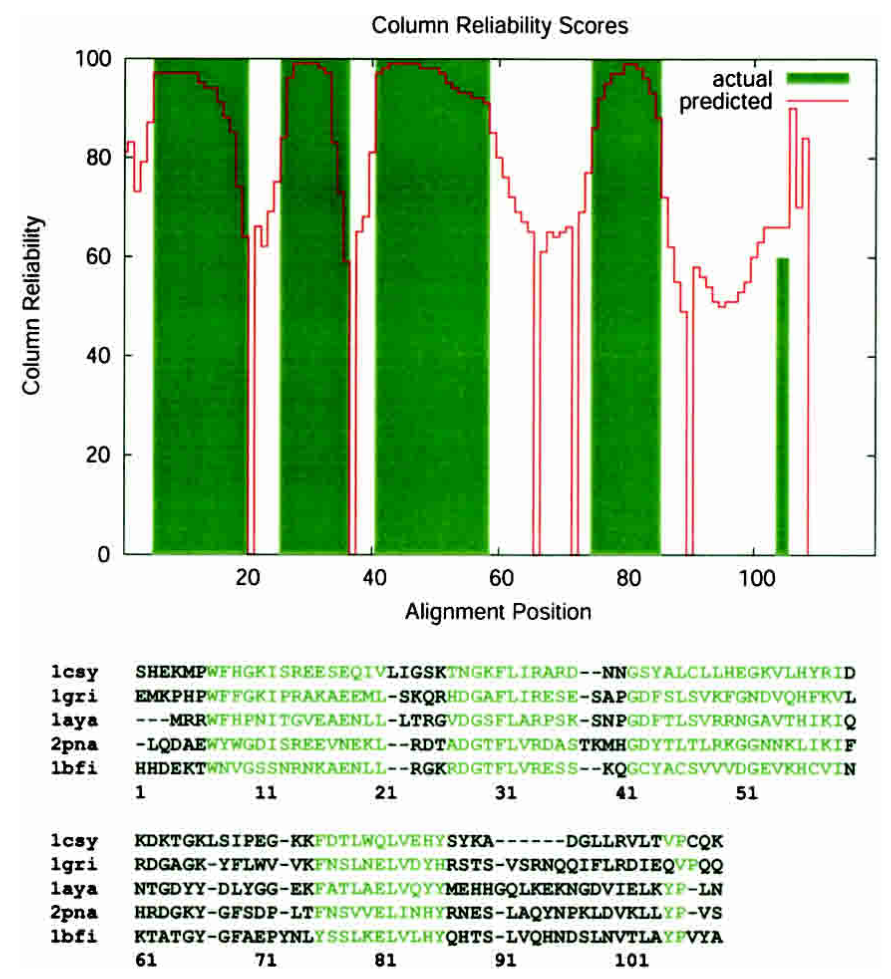
\includegraphics[width=0.6\textheight]{img/exp1.png}
            \end{figure}
        \column{0.47\textwidth}
            \textbf{Image from \cite{do2005probcons}.} 

            At each position:
            \begin{itemize}
                \item Red line $\rightarrow$ predicted proportion of correct pairwise matches.
                \item Green Blocks $\rightarrow$ actual proportion of correct pairwise matches.
            \end{itemize}
    \end{columns}
\end{frame}

\begin{frame}
    \frametitle{Comparison with other methods}
    \begin{figure}[t]
        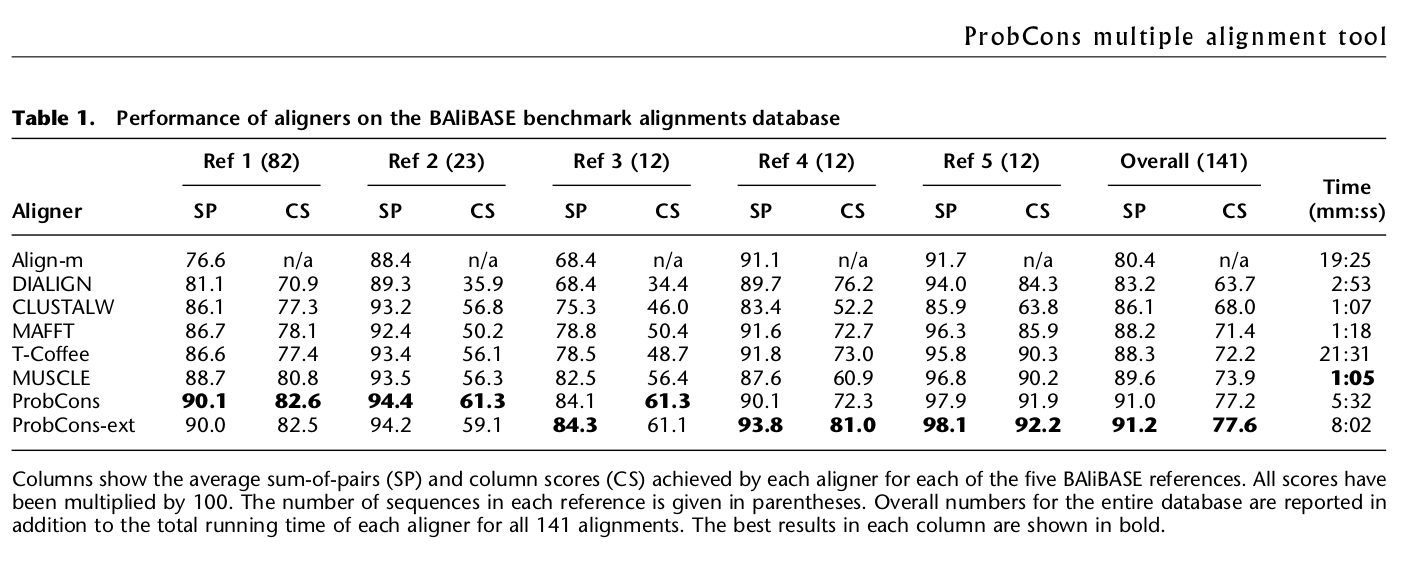
\includegraphics[width=0.9\textwidth]{img/exp2.png}
        \caption{Image from \cite{do2005probcons}.}
    \end{figure}
\end{frame}

\section{Example} 
\begin{frame}{Examples: Comparison between methods}

    \begin{itemize}
        \item MSA of distantly related globins (human beta globin, human myoglobin, human neuroglobin, soybean leghemoglobin, rice hemoglobin) using four different programs. Symbols: * complete conservation, : conservative substitutions, . less conservative substitutions. Programs differ in:
        \begin{itemize}
            \item Align corresponding regions of alpha helical secondary structure (red lettering).
            \item Align conserved histidines (open and black arrowhead). They are important in coordinating protein binding to the heme group $\rightarrow$ they should be aligned by all the programs. The open arrowhead histidine shows a complete conservation. The conservation of the black is only achieved by ProbCons and T-Coffee.
            \item Create and place gaps (boxed regions).
        \end{itemize}
    \end{itemize}
            
\end{frame}

\begin{frame}

    \begin{figure}[t]
        \raggedleft
        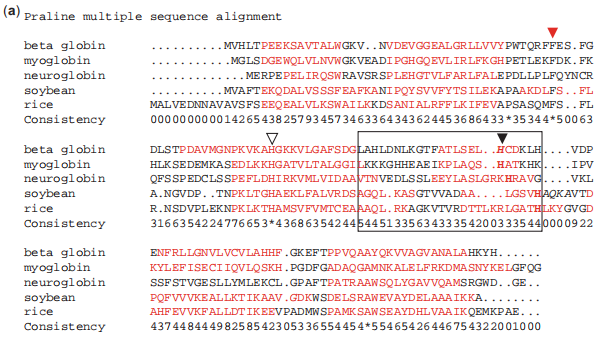
\includegraphics[width=0.49\textwidth]{./img/Comparacion_1.png}
        \raggedright
        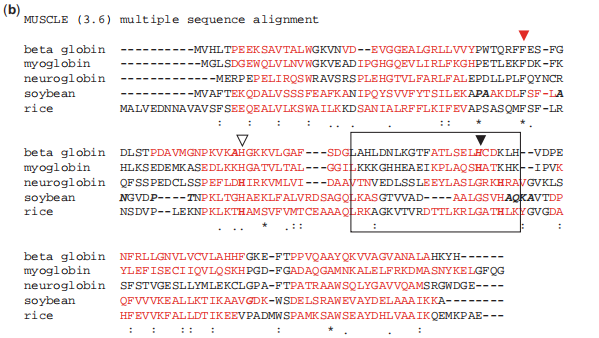
\includegraphics[width=0.49\textwidth]{./img/Comparacion_2.png}
    \end{figure}
    \begin{figure}[b]
        \raggedleft
        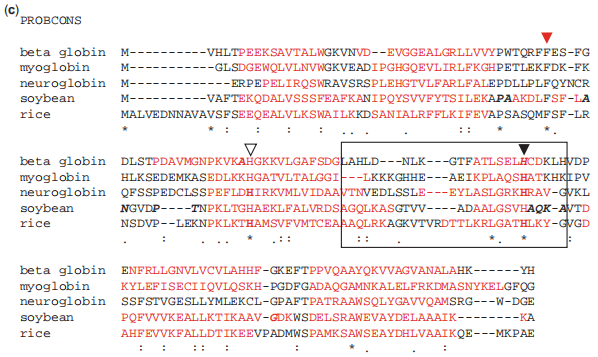
\includegraphics[width=0.49\textwidth]{./img/Comparacion_3.png}
        \raggedright
        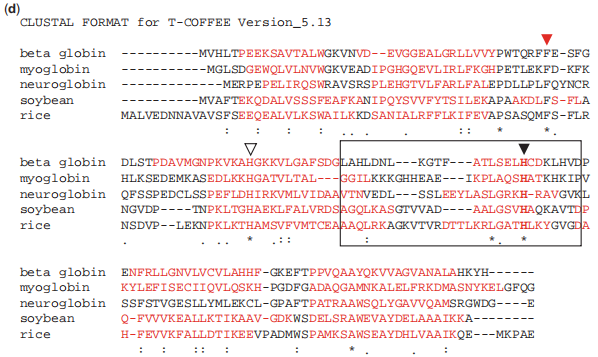
\includegraphics[width=0.49\textwidth]{./img/Comparacion_4.png}
    \end{figure}

\end{frame}

\section{Drawbacks and Conclusions}
\begin{frame}{Drawbakcs}
    \begin{itemize}
        \item \textbf{Computational weight:} The computation step of calculation of posterior probabilities  takes time $O(m^2L^2)$, where m is the number of sequences and L is the length of each sequence.
        \item \textbf{M-Coffe (Meta-Coffe):} combines the output of 15 different sequence alignment methods(ProbCons included). M-Coffe employs a consistency-based approach to estimate a more accurate consensus alignment. 
        \item \textbf{Structural methods:} adding structural information, even further accuracy is achieved. 
    \end{itemize}
    
\end{frame}
\begin{frame}{Conclusions}
The ProbCons algorithm uses an extremely simple model of sequence similarity (a three-state pair-HMM):
    \begin{enumerate}
        \item Makes no attempt to incorporate biological knowledge (i.e position specific gap scoring or rigorous evolutionary tree construction).
        \item Use amino acid alphabet and BLOSUM emission probability matrices as protein-specific alignment information.
        \item Can be used to DNA alignment by changing the alphabet and the BLOSUM matrices with values for nucleotides.
        \item The parameter used in the model are transparent ($\pi_{insert}$, $\delta$, $\epsilon$).
        \item The training program is done automatically on unaligned sequences using Expectation-Maximization.
        \item High accuracy: probabilistic consistency transformation and objective function. 
    \end{enumerate}
\end{frame}



\section{References}
\begin{frame}[allowframebreaks]
    \frametitle{References}
    \bibliographystyle{amsalpha}
    \bibliography{files/bibliografia.bib}
\end{frame}



%%%%%%%% greetings %%%%%%%%
\frame{\titlepage}
%------------------------------------------------



\end{document}